\section{Background}
\label{sec:background}

This section states the results the design rule builds on; full derivations are in the
repository's derivations folder.

\subsection{Classical side}

\textbf{PINNs.} A PINN \citep{raissi2019pinn} minimises the PDE residual at sampled
collocation points, with derivatives from automatic differentiation that are exact to
floating-point precision. Unlike a Galerkin or finite-element method, the optimisation is
non-convex in the network parameters even when the PDE is linear.

\textbf{The NTK and spectral bias.} Writing
$\Theta(x,x')=\nabla_\theta N[u_\theta](x)\cdot\nabla_\theta N[u_\theta](x')^\top$ for the
residual's tangent kernel \citep{jacot2018ntk}, gradient-flow training in the lazy regime
linearises to $\dot e = -\Theta_0 e$, so each eigenmode of $\Theta_0$ decays as
$\exp(-\lambda_i t)$. For a tanh or ReLU MLP the eigenvalues decay roughly as a power law
in Fourier-mode index, so high-frequency components are learned last and slowly
(Figure~\ref{fig:staircase}). Fourier-feature encodings \citep{tancik2020fourier} are the
standard classical fix, and therefore a necessary baseline: a quantum layer that beats
only a plain MLP has bought nothing Fourier features do not already supply.

\begin{figure}[htbp]
  \centering
  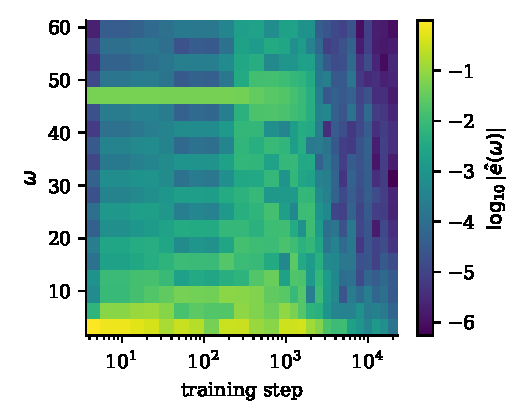
\includegraphics[width=0.45\linewidth]{figures/staircase_cmlp_p1.pdf}
  \caption{Spectral bias, measured: per-frequency error of a plain MLP over training on
    the Poisson problem, $u^*=\sin(\pi x)+\alpha\sin(15\pi x)$ with $\alpha=0.05$. The
    $\omega=\pi$ mode converges first; $\omega=15\pi\approx47$ needs 16.2 times as many
    steps to reach tolerance (3 seeds).}
  \label{fig:staircase}
\end{figure}

\textbf{Hard boundary conditions.} The ansatz $u = B(x) + D(x)\,N(x)$, with $D$ vanishing
on the boundary and $B$ matching the boundary data, satisfies the boundary conditions by
construction and removes the boundary-loss block of the NTK.

\subsection{Quantum side}

\textbf{Re-uploading circuits are Fourier series.} For encoding gates $\exp(-ix H^{(l)})$
with generator eigenvalues $\{\lambda^{(l)}_a\}$, an $L$-layer re-uploading circuit's
output is a truncated Fourier series whose frequencies are the signed sums of per-layer
eigenvalue differences \citep{schuld2021effect}. This is the fact SMCD engineers on
(Proposition~1).

\textbf{Exact derivatives on hardware.} The parameter-shift rule
$\partial_\theta f = \tfrac12[f(\theta+\pi/2) - f(\theta-\pi/2)]$ holds for Pauli-generated
gates, and because the input $x$ enters as a rotation angle, $\partial_x f$ is also exact
by a shift. The PINN residual can therefore be computed exactly on quantum hardware, not
only in simulation.

\textbf{Barren plateaus.} $\mathrm{Var}[\partial_\theta C]$ decays exponentially in qubit
count for a global cost on a deep random circuit \citep{mcclean2018barren}. SMCD avoids
this by construction: the depth rule picks the \emph{minimum} depth that covers the target
band, the observable is local, and angles start small.

\textbf{Effective dimension.} The effective dimension of \citet{abbas2021effdim}, from the
empirical Fisher spectrum, measures capacity beyond parameter count and is reported for
every family.
